
%----------------------------------------------------------------------------------------
%	PACKAGES AND DOCUMENT CONFIGURATIONS
%----------------------------------------------------------------------------------------

\documentclass{article}

\usepackage[version=3]{mhchem} % Package for chemical equation typesetting
\usepackage{siunitx} % Provides the \SI{}{} and \si{} command for typesetting SI units
\usepackage{graphicx} % Required for the inclusion of images
\usepackage{natbib} % Required to change bibliography style to APA
\usepackage{amsmath} % Required for some math elements
\usepackage{multirow}
\usepackage{listings}
\usepackage{moreverb} 
\usepackage{vmargin}
\usepackage{float}
\usepackage{fancyhdr}

\setpapersize{USletter}
\setmarginsrb{1in}{0.5in}{1in}{0.2in}{12pt}{11mm}{0pt}{11mm}

%----------------------------------------------------------------------------------------
%	DOCUMENT INFORMATION
%----------------------------------------------------------------------------------------

\title{Fitbrick S\\ BME 354L}
\author{Matias \textsc{Lopez}, Raiyan \textsc{Sobhan}}
\date{\today}

\pagestyle{fancy}
\rhead{Matias Lopez, Raiyan Sobhan}
\lhead{BME 354L}


\begin{document}

\maketitle % Insert the title, author and date

\begin{center}
\begin{tabular}{l r}
Last Revision: & December 2, 2015 \\
TA: & Ningrui Li % Instructor/supervisor
\end{tabular}
\end{center}

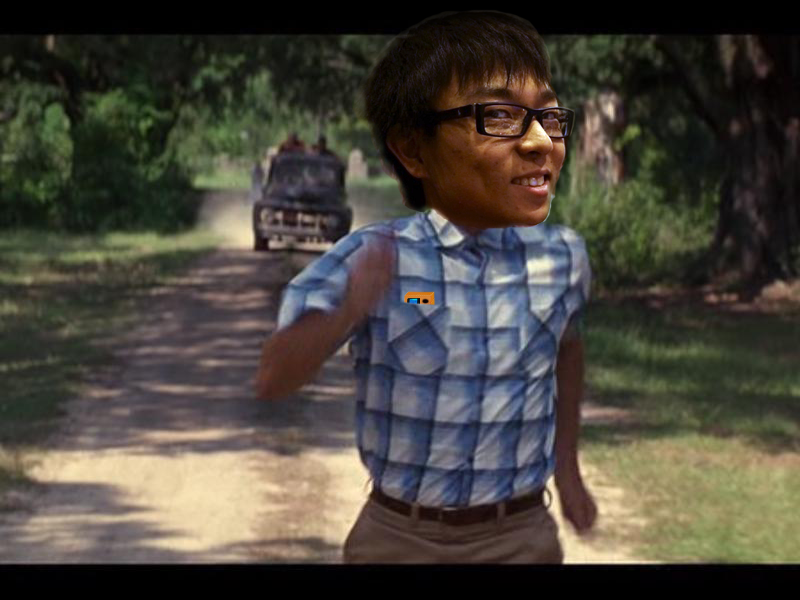
\includegraphics[width=5.5in]{ningrui}

\section*{Table of Contents}
\tableofcontents

\pagebreak

%----------------------------------------------------------------------------------------
%	SECTION 1
%----------------------------------------------------------------------------------------
\section{What's Included}
Your new \textbf{\textit{FitBrick S}} will help you attain all your fitness goals. It keeps track of your walking so you don't have to!  Wearing the \textbf{\textit{FitBrick S}} allows you to keep track of your daily activity. Locally stored data lets you see your short term activities for each battery cycle. 

Included in the box are:\\
\begin{tabular}{l l c}
	1 & USB to USB Mini B Cord & \multirow{5}{*}{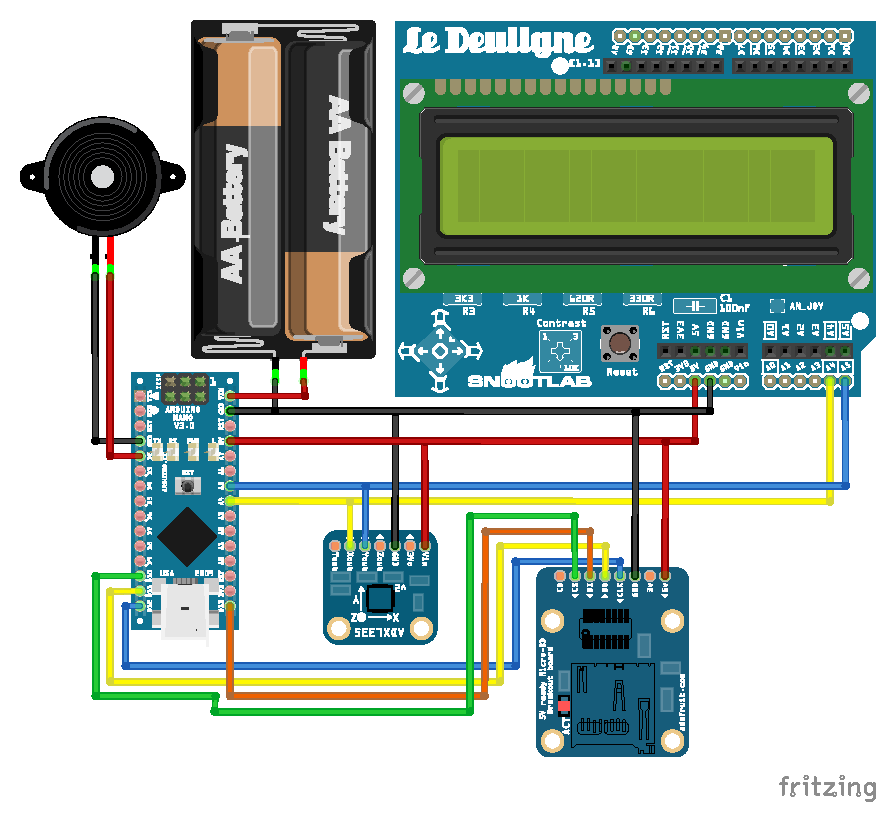
\includegraphics[width=2.0in]{sketch_bb}}\\
	4 & Rechargeable 1.2V Batteries* & ~\\
	1 & \textbf{\textit{FitBrick S}} & ~\\
	1 & Micro SD Card  & ~ \\
	1 & Micro SD to SD Adaptor & ~
\end{tabular}
\\
* Charger not included.
\section{Quick Start Guide}
\subsection{Daily Setup}
Unscrew the back cover of the \textbf{\textit{FitBrick S}}. Charge and place the provided batteries into the battery slots and ensure that no wires have fallen out (wiring scheme shown above). Screw the back cover back onto the \textbf{\textit{FitBrick S}}. The \textbf{\textit{FitBrick S}} will now track your activity for the next 8 or more hours. For best accuracy, the \textbf{\textit{FitBrick S}} should be work in either leg.

\subsection{\textbf{\textit{FitBrick S}} Functions}
On all screens, the lifetime steps for each user (as determined by which Micro SD card is in the unit) will be displayed in the lower lefthand corner. The lower righthand corner of the screen will display a number of hashmarks (\#) corresponding to the current activity level: level 1 is less than 120 steps per minute, level 2 is less than 160 steps per minute, and level 3 is more than 160 steps per minute. \\
The default screen (shown below) will display the number of steps taken since the last reset in the upper lefthand corner. This count can be reset by hitting the SELECT button. \\
Hitting the RIGHT button will change the top line to display acceleration data in three axes, given in units of percent of 1\textit{g}, the acceleration due to gravity. \\
Hitting the UP button will activate Trainer Mode. In this mode, the user sets an activity level (1, 2, or 3 as defined above) that they wish to exercise at. The DOWN button decrements the activity level. If the user activity falls below this level, the \textbf{\textit{FitBrick S}} will beep until the proper activity level is reached. 
\subsection{Data Recovery}
Unscrew the back cover of the \textbf{\textit{FitBrick S}} and remove the Micro SD card. Place the Micro SD card into the provided Micro SD to SD Adaptor and place the adaptor into a computer. All data should be stored in a file called 'FBRCKLOG.csv'. 
\begin{center}
	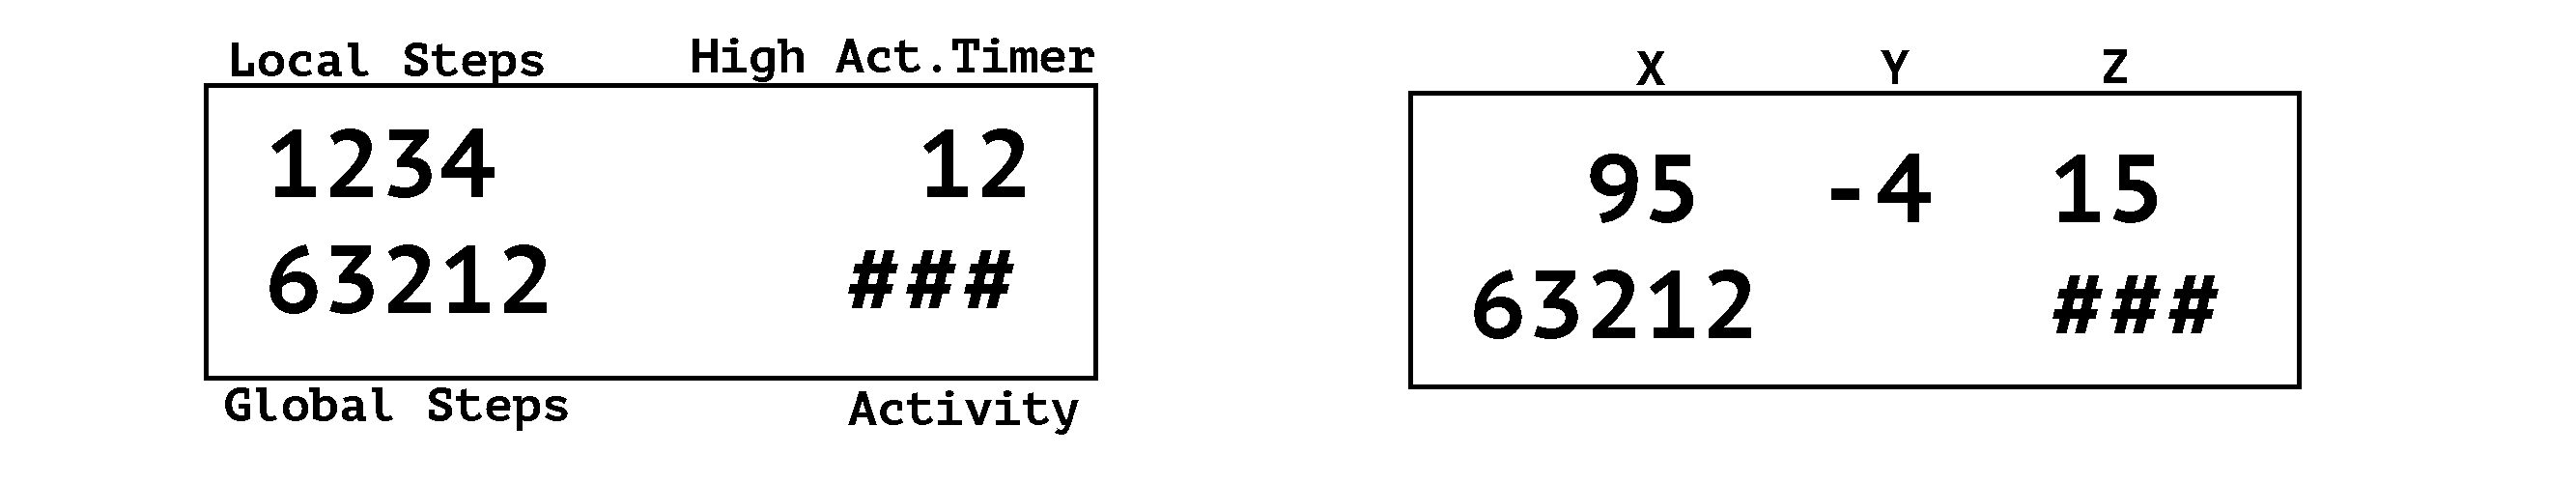
\includegraphics[width=6.5in]{screen}
\end{center}
%----------------------------------------------------------------------------------------
%	BIBLIOGRAPHY
%----------------------------------------------------------------------------------------

\bibliographystyle{apalike}

\bibliography{sample}

%----------------------------------------------------------------------------------------


\end{document}